% SPDX-License-Identifier: CC-BY-SA-4.0
%
% Copyright (C) 2026 embedded brains GmbH & Co. KG
\documentclass[tikz,border=4pt]{standalone}
\usepackage[T1]{fontenc}
\usepackage[scaled]{helvet}
\renewcommand{\familydefault}{\sfdefault}
\usetikzlibrary{arrows.meta,backgrounds,positioning,calc}
\definecolor{ebblue}{HTML}{1F4E79}
\definecolor{boxfill}{HTML}{EAF1F8}
\definecolor{codefill}{HTML}{FFF4E0}
\definecolor{codeline}{HTML}{9C6500}
\definecolor{groupfill}{HTML}{F5F5F5}
\definecolor{flow}{HTML}{404040}
\begin{document}
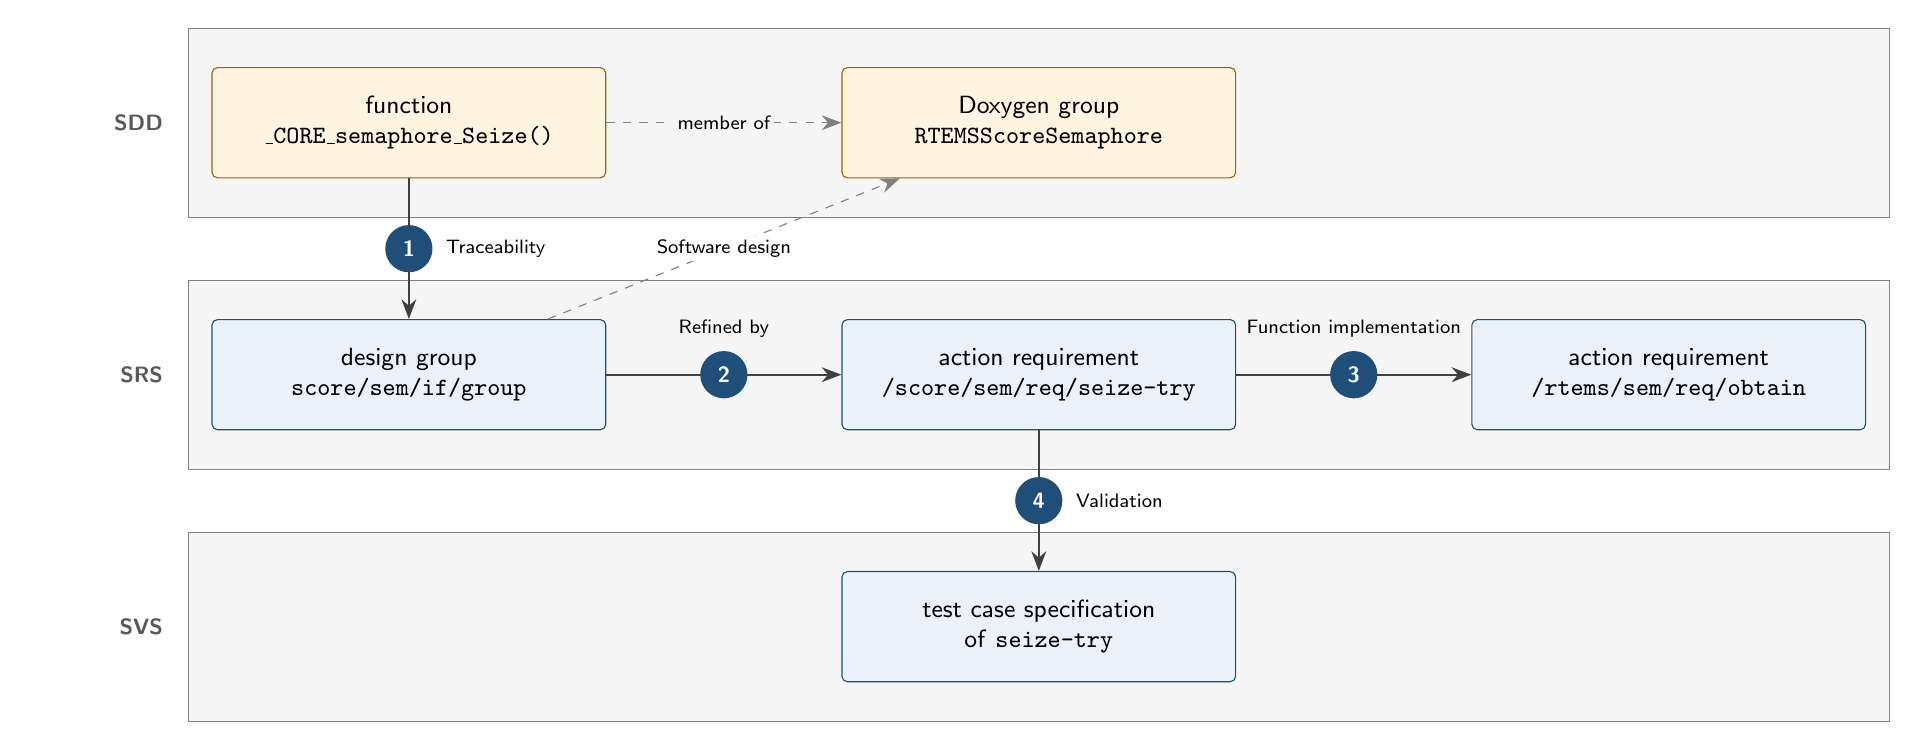
\begin{tikzpicture}[
    font=\small,
    doc/.style={draw=ebblue, fill=boxfill, rounded corners=2pt,
      minimum width=50mm, minimum height=14mm, align=center},
    sdd/.style={draw=codeline, fill=codefill, rounded corners=2pt,
      minimum width=50mm, minimum height=14mm, align=center},
    edge/.style={-{Stealth[length=2.5mm]}, thick, draw=flow},
    back/.style={-{Stealth[length=2.5mm]}, thin, dashed, draw=gray},
    lbl/.style={font=\scriptsize, align=center, fill=groupfill, inner sep=1.5pt},
    stepno/.style={circle, fill=ebblue, text=white, font=\footnotesize\bfseries,
      inner sep=0pt, minimum size=6mm},
    steplbl/.style={font=\scriptsize, align=left, inner sep=1.5pt},
    lanelabel/.style={font=\footnotesize\bfseries, text=gray!70!black,
      align=right, anchor=east, text width=16mm}]

  \def\left{-1.2}\def\right{20.4}
  \foreach \y/\name in {3.2/SDD, 0/SRS, -3.2/SVS} {
    \fill[groupfill] (\left,\y-1.2) rectangle (\right,\y+1.2);
    \draw[gray] (\left,\y-1.2) rectangle (\right,\y+1.2);
    \node[lanelabel] at (\left-0.2,\y) {\name};
  }

  \node[sdd] (unit) at (1.6,3.2)
    {function\\\texttt{\_CORE\_semaphore\_Seize()}};
  \node[doc] (group) at (1.6,0)
    {design group\\\texttt{score/sem/if/group}};
  \node[doc] (try) at (9.6,0)
    {action requirement\\\texttt{/score/sem/req/seize-try}};
  \node[doc] (obtain) at (17.6,0)
    {action requirement\\\texttt{/rtems/sem/req/obtain}};
  \node[doc] (spec) at (9.6,-3.2)
    {test case specification\\of \texttt{seize-try}};
  \node[sdd] (doxgroup) at (9.6,3.2)
    {Doxygen group\\\texttt{RTEMSScoreSemaphore}};

  \draw[edge] (unit) -- node[stepno] (s1) {1} (group);
  \node[steplbl, right=1mm of s1] {Traceability};
  \draw[edge] (group) -- node[stepno] (s2) {2} (try);
  \node[steplbl, above=1mm of s2] {Refined by};
  \draw[edge] (try) -- node[stepno] (s3) {3} (obtain);
  \node[steplbl, above=1mm of s3] {Function implementation};
  \draw[edge] (try) -- node[stepno] (s4) {4} (spec);
  \node[steplbl, right=1mm of s4] {Validation};
  \draw[back] (group) -- node[lbl, pos=0.5, fill=white] {Software design} (doxgroup);
  \draw[back] (unit) -- node[lbl] {member of} (doxgroup);
\end{tikzpicture}
\end{document}
